\documentclass[11pt,a4paper]{article}
\usepackage[margin=2.2cm]{geometry}
\usepackage{amsmath,amssymb,booktabs,graphicx,enumitem,xcolor,array}
\usepackage[hidelinks]{hyperref}
\usepackage[font=small,labelfont=bf]{caption}
\setlength{\parskip}{4pt}\setlength{\parindent}{0pt}
\newcommand{\TODO}[1]{\textcolor{red}{[#1]}}
\IfFileExists{../team_private.tex}{\input{../team_private.tex}}{% Team details, shared by the proposal, the progress report and the final report.
% Fill in the names once here. For the printed submission, copy this file to team_private.tex
% (git-ignored) and add student IDs there; the reports use team_private.tex when it exists.
\providecommand{\TODO}[1]{\textcolor{red}{[#1]}}
\newcommand{\TeamNames}{Nguyen Van Thanh, \TODO{Member 2}, \TODO{Member 3}, \TODO{Member 4}, \TODO{Member 5}}
\newcommand{\TeamNamesStacked}{Nguyen Van Thanh\\ \TODO{Member 2} \quad \TODO{Member 3} \quad \TODO{Member 4} \quad \TODO{Member 5}}
% owner of each method (one method per member)
\newcommand{\MOne}{\TODO{Member A}}
\newcommand{\MTwo}{\TODO{Member B}}
\newcommand{\MThree}{\TODO{Member C}}
\newcommand{\MFour}{\TODO{Member D}}
\newcommand{\MFive}{\TODO{Member E}}
\newcommand{\SubmissionDate}{\TODO{Submission date}}
}

\begin{document}
\begin{center}
{\large Operations Research 76000093 --- Final Project Proposal}\\[6pt]
{\LARGE\bfseries Right Place, Right Time:\\[2pt] Optimizing Public EV Charging Capacity, Guidance and Pricing in Shenzhen}\\[8pt]
Team members: \TeamNames
\end{center}

\section{What we will study, and why it matters}
Shenzhen is one of the world's most electrified cities: by June 2024 it had 1.08 million new-energy vehicles, more than 25\% of its 4.26 million vehicles~\cite{cnev2024}. Public charging piles are the bottleneck for drivers without home charging (taxis, ride-hailing and many residents). A charging network can fail in two ways. Piles in the wrong places leave drivers queueing in one district while piles stand idle in the next. Piles used at the wrong times sit empty all afternoon and saturate at night.

We will use the open \textbf{UrbanEV} dataset~\cite{li2025urbanev}: hourly occupancy, charging duration, energy and prices of \textbf{17{,}532 public piles at 1{,}362 stations in 275 traffic zones} of Shenzhen (Sep 2022--Feb 2023, CC0 licence). A first look at the data already shows the mismatch (Fig.~\ref{fig:prelim}):
\begin{itemize}[leftmargin=1.3em,itemsep=1pt]
\item \textbf{Low average use, but local saturation.} The network-wide occupancy is only 28\%, peaking at night (0--6 h, cheap valley tariff). On the busiest 10\% of days, however, 10 zones have \emph{all} piles occupied.
\item \textbf{Growth will break the network.} China's NEV stock grew by 49\% in the year to June 2025~\cite{cnev2025}. With charging demand doubled and the current piles, a first M/M/$c$ queueing analysis finds \textbf{48 zones with unstable queues}, although network-wide occupancy would still be only 56\%.
\end{itemize}
The problem is therefore not simply ``build more piles''. It is a joint allocation problem in space (\emph{where}) and time (\emph{when}), with several levers of very different cost: new piles, relocating idle piles, guiding drivers to nearby zones, and time-of-use prices. This makes it a natural and realistic operations research problem, with public data, a clear decision maker (city planners and charging operators) and measurable outcomes (driver waiting time, investment).

\begin{figure}[h]\centering
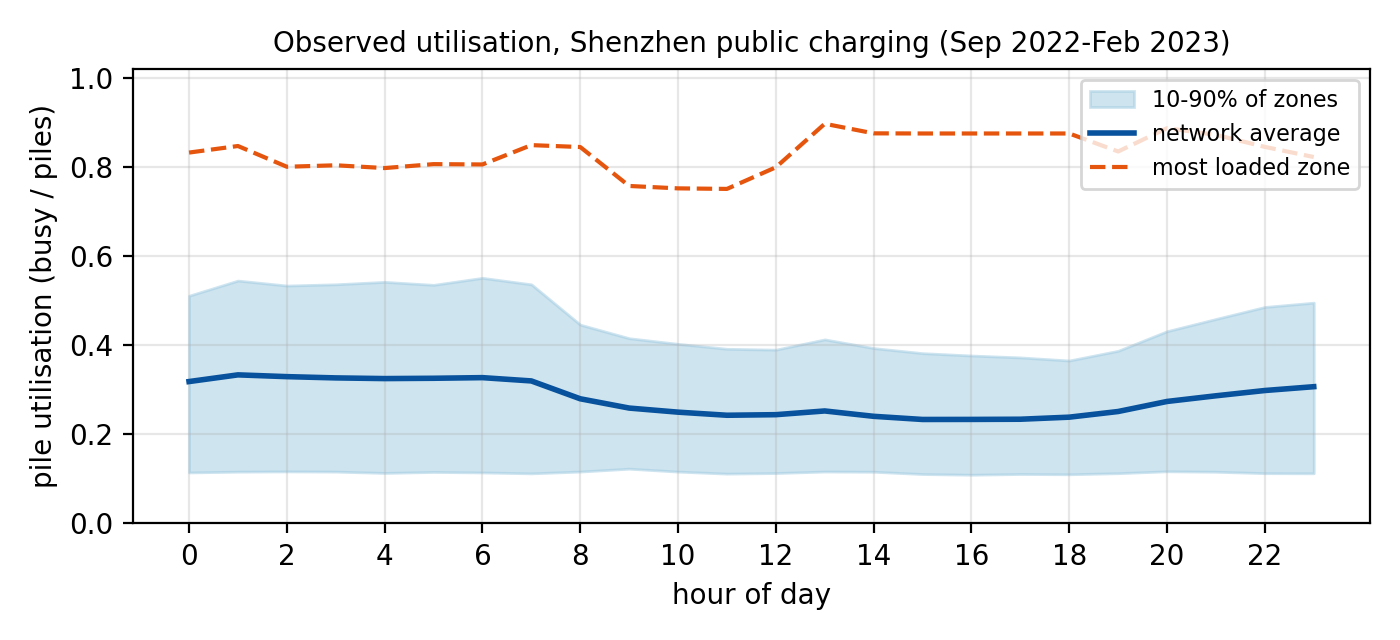
\includegraphics[width=0.49\linewidth]{../../figures/m1_hourly_util.png}\hfill
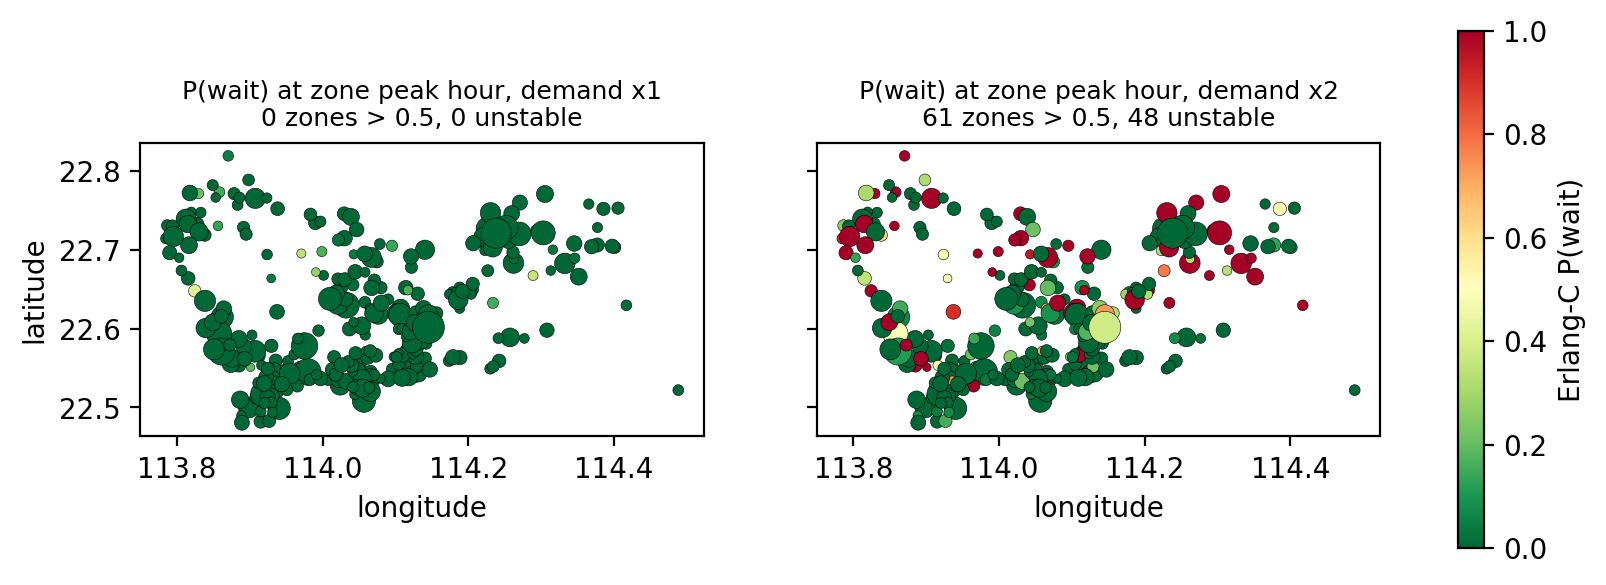
\includegraphics[width=0.49\linewidth]{../../figures/m1_map_pwait.png}
\caption{Preliminary evidence. Left: hourly pile utilisation (observed). Right: Erlang-C probability of waiting at each zone's peak hour for current demand (left panel) and doubled demand (right panel); marker size is the number of piles.}\label{fig:prelim}
\end{figure}

\section{Objectives and research questions}
\textbf{Objective:} minimise total driver waiting time in the Shenzhen public charging network under demand growth, at the lowest investment. We will answer five questions, each with one method from the course (one per team member):
\begin{enumerate}[label=\textbf{RQ\arabic*},leftmargin=2.8em,itemsep=1pt]
\item How long do drivers wait in each zone and hour, and which zones fail first as demand grows? --- \emph{queueing theory}.
\item Given a budget, where should new piles be installed and idle piles relocated? --- \emph{integer programming}.
\item How much overload can navigation guidance absorb, by redirecting drivers to nearby zones without building anything? --- \emph{network optimisation}.
\item Which revenue-neutral time-of-use service fee shifts charging away from congested hours? --- \emph{nonlinear programming}.
\item Do the analytical models hold when demand varies over the day and drivers spill over to neighbouring zones, and can a simulation-based search do better? --- \emph{simulation and metaheuristics}.
\end{enumerate}

\section{Methods (one per member)}
\begin{tabular}{@{}p{3.1cm}p{12.6cm}@{}}
\toprule
\textbf{M1 Queueing} & Each zone is modelled as an M/M/$c$ system with $c$ piles and hourly offered load $a_{zh}$ (Erlangs) estimated from the data. We compute $P(\text{wait})$ with Erlang-C and total waiting time $\sum_h \lambda W_q$, and derive stability thresholds and growth scenarios.\\
\textbf{M2 Integer programming} & Budget-constrained expansion and relocation. The waiting cost is convex in the number of piles, so it can be linearised exactly with 0-1 increment variables; the model is a MILP with a budget constraint and a stability constraint for every zone. Duality and sensitivity analysis give the shadow price of the budget and the break-even relocation cost.\\
\textbf{M3 Network optimisation} & A min-cost flow (transportation) model redirects excess demand from overloaded zones to zones with spare capacity within a detour limit. We solve it with LP and the network simplex method and analyse the trade-off between detour limit and resolved overload.\\
\textbf{M4 Nonlinear programming} & Drivers choose their charging hour by a logit model; price sensitivity is estimated from zones with and without time-of-use prices. We then optimise a 24-hour fee profile under revenue neutrality, with KKT conditions and Lagrange-multiplier interpretation.\\
\textbf{M5 Simulation + metaheuristic} & A discrete-event simulation with time-varying arrivals, general session lengths and driver spill-over, verified against Erlang-C. Simulated annealing then searches pile allocations with common random numbers, and plans are compared out of sample.\\
\bottomrule
\end{tabular}

The results of the five methods will be combined into a policy portfolio: pricing + guidance + investment, compared on the same metric of budget needed to reach a waiting-time target.

\section{Related literature (at least 5 papers will be reviewed)}
Charging and refuelling location models build on the flow-capturing and flow-refuelling models~\cite{hodgson1990,kuby2005}. Equilibrium-based deployment of public charging is studied in~\cite{he2013}. Queueing delay has been embedded in charger siting for electric taxis through bi-level simulation-optimisation~\cite{jung2014} and M/M/$x$/$s$-based integer programs~\cite{yang2017}. For time-varying demand, the SIPP staffing approach and its limitations~\cite{green2001} motivate our simulation check. Marginal analysis for separable convex resource allocation~\cite{fox1966} underpins our incremental MILP. On the data side, UrbanEV~\cite{li2025urbanev} and its companion studies on price effects~\cite{kuang2024} and demand prediction~\cite{qu2024} give the empirical basis.

\section{Work plan, milestones and task allocation}
\begin{tabular}{@{}p{3.3cm}p{12.4cm}@{}}\toprule
\textbf{Date} & \textbf{Milestone}\\\midrule
Oct 26 & Proposal submitted; data pipeline and preliminary queueing results (done).\\
Nov 2--15 & M1--M5 base models implemented and verified (formula checks, solver cross-checks, simulation vs Erlang-C).\\
Nov 16--29 & Literature review (at least 5 papers), sensitivity analyses (growth, relocation cost, detour limit, price sensitivity).\\
Nov 30 & \textbf{Progress report} (hardcopy): problems, methods and rationale, preliminary results, schedule.\\
Dec 1--(TBA) & Integrated policy portfolio, final analysis, final report, 10--15 slides, rehearsal (every member presents their method).\\
(TBA) & \textbf{Final report} (hardcopy + ZIP of code, data, results, slides on Web Learning) and \textbf{presentation}.\\\bottomrule
\end{tabular}

\medskip
\begin{tabular}{@{}p{4.2cm}p{11.5cm}@{}}\toprule
\textbf{Member} & \textbf{Responsibility}\\\midrule
\MOne & M1 queueing model, demand estimation from data, growth scenarios; data pipeline.\\
\MTwo & M2 MILP expansion/relocation, duality and sensitivity analysis.\\
\MThree & M3 min-cost-flow guidance model, network simplex cross-check.\\
\MFour & M4 logit price-sensitivity estimation, NLP fee design, KKT analysis.\\
\MFive & M5 discrete-event simulation, simulated annealing, out-of-sample validation.\\
All & Literature review (two papers each), integrated policy analysis, report writing, slides.\\\bottomrule
\end{tabular}

\textbf{Team size.} The guidelines specify 3--4 students; our team has five. We request the instructor's approval. Following the rule of one method per member, we commit to five distinct methods.

\begin{thebibliography}{99}\small
\bibitem{li2025urbanev} H.~Li, H.~Qu, X.~Tan, L.~You, R.~Zhu, W.~Fan, ``UrbanEV: An open benchmark dataset for urban electric vehicle charging demand prediction,'' \emph{Scientific Data}, 12:523, 2025. doi:10.1038/s41597-025-04874-4.
\bibitem{kuang2024} H.~Kuang, X.~Zhang, H.~Qu, L.~You, R.~Zhu, J.~Li, ``Unraveling the effect of electricity price on electric vehicle charging behavior: A case study in Shenzhen, China,'' \emph{Sustainable Cities and Society}, 115:105836, 2024. doi:10.1016/j.scs.2024.105836.
\bibitem{qu2024} H.~Qu, H.~Kuang, Q.~Wang, J.~Li, L.~You, ``A physics-informed and attention-based graph learning approach for regional electric vehicle charging demand prediction,'' \emph{IEEE Trans.\ Intelligent Transportation Systems}, 25(10):14284--14297, 2024. doi:10.1109/TITS.2024.3401850.
\bibitem{hodgson1990} M.~J.~Hodgson, ``A flow-capturing location-allocation model,'' \emph{Geographical Analysis}, 22(3):270--279, 1990.
\bibitem{kuby2005} M.~Kuby, S.~Lim, ``The flow-refueling location problem for alternative-fuel vehicles,'' \emph{Socio-Economic Planning Sciences}, 39(2):125--145, 2005.
\bibitem{he2013} F.~He, D.~Wu, Y.~Yin, Y.~Guan, ``Optimal deployment of public charging stations for plug-in hybrid electric vehicles,'' \emph{Transportation Research Part B}, 47:87--101, 2013.
\bibitem{jung2014} J.~Jung, J.~Y.~J.~Chow, R.~Jayakrishnan, J.~Y.~Park, ``Stochastic dynamic itinerary interception refueling location problem with queue delay for electric taxi charging stations,'' \emph{Transportation Research Part C}, 40:123--142, 2014.
\bibitem{yang2017} J.~Yang, J.~Dong, L.~Hu, ``A data-driven optimization-based approach for siting and sizing of electric taxi charging stations,'' \emph{Transportation Research Part C}, 77:462--477, 2017.
\bibitem{green2001} L.~V.~Green, P.~J.~Kolesar, J.~Soares, ``Improving the SIPP approach for staffing service systems that have cyclic demands,'' \emph{Operations Research}, 49(4):549--564, 2001.
\bibitem{fox1966} B.~Fox, ``Discrete optimization via marginal analysis,'' \emph{Management Science}, 13(3):210--216, 1966.
\bibitem{cnev2024} CnEVPost, ``Shenzhen NEV penetration reaches record 77.4\% in Jun,'' Jul.~18, 2024. \url{https://cnevpost.com/2024/07/18/shenzhen-nev-penetration-jun-2024/}
\bibitem{cnev2025} CnEVPost, ``China NEV ownership reaches 36.89 million,'' Jul.~14, 2025 (24.72 million in Jun 2024). \url{https://cnevpost.com/2025/07/14/china-nev-ownership-36-89-million-jun-2025/}
\end{thebibliography}
\end{document}
